\documentclass[]{article}
\usepackage{lmodern}
\usepackage{amssymb,amsmath}
\usepackage{ifxetex,ifluatex}
\usepackage{fixltx2e} % provides \textsubscript
\ifnum 0\ifxetex 1\fi\ifluatex 1\fi=0 % if pdftex
  \usepackage[T1]{fontenc}
  \usepackage[utf8]{inputenc}
\else % if luatex or xelatex
  \ifxetex
    \usepackage{mathspec}
  \else
    \usepackage{fontspec}
  \fi
  \defaultfontfeatures{Ligatures=TeX,Scale=MatchLowercase}
\fi
% use upquote if available, for straight quotes in verbatim environments
\IfFileExists{upquote.sty}{\usepackage{upquote}}{}
% use microtype if available
\IfFileExists{microtype.sty}{%
\usepackage{microtype}
\UseMicrotypeSet[protrusion]{basicmath} % disable protrusion for tt fonts
}{}
\usepackage[margin=1in]{geometry}
\usepackage{hyperref}
\hypersetup{unicode=true,
            pdftitle={Environ 710 HW 11},
            pdfauthor={Natalia Neal-Walthall},
            pdfborder={0 0 0},
            breaklinks=true}
\urlstyle{same}  % don't use monospace font for urls
\usepackage{color}
\usepackage{fancyvrb}
\newcommand{\VerbBar}{|}
\newcommand{\VERB}{\Verb[commandchars=\\\{\}]}
\DefineVerbatimEnvironment{Highlighting}{Verbatim}{commandchars=\\\{\}}
% Add ',fontsize=\small' for more characters per line
\usepackage{framed}
\definecolor{shadecolor}{RGB}{248,248,248}
\newenvironment{Shaded}{\begin{snugshade}}{\end{snugshade}}
\newcommand{\KeywordTok}[1]{\textcolor[rgb]{0.13,0.29,0.53}{\textbf{#1}}}
\newcommand{\DataTypeTok}[1]{\textcolor[rgb]{0.13,0.29,0.53}{#1}}
\newcommand{\DecValTok}[1]{\textcolor[rgb]{0.00,0.00,0.81}{#1}}
\newcommand{\BaseNTok}[1]{\textcolor[rgb]{0.00,0.00,0.81}{#1}}
\newcommand{\FloatTok}[1]{\textcolor[rgb]{0.00,0.00,0.81}{#1}}
\newcommand{\ConstantTok}[1]{\textcolor[rgb]{0.00,0.00,0.00}{#1}}
\newcommand{\CharTok}[1]{\textcolor[rgb]{0.31,0.60,0.02}{#1}}
\newcommand{\SpecialCharTok}[1]{\textcolor[rgb]{0.00,0.00,0.00}{#1}}
\newcommand{\StringTok}[1]{\textcolor[rgb]{0.31,0.60,0.02}{#1}}
\newcommand{\VerbatimStringTok}[1]{\textcolor[rgb]{0.31,0.60,0.02}{#1}}
\newcommand{\SpecialStringTok}[1]{\textcolor[rgb]{0.31,0.60,0.02}{#1}}
\newcommand{\ImportTok}[1]{#1}
\newcommand{\CommentTok}[1]{\textcolor[rgb]{0.56,0.35,0.01}{\textit{#1}}}
\newcommand{\DocumentationTok}[1]{\textcolor[rgb]{0.56,0.35,0.01}{\textbf{\textit{#1}}}}
\newcommand{\AnnotationTok}[1]{\textcolor[rgb]{0.56,0.35,0.01}{\textbf{\textit{#1}}}}
\newcommand{\CommentVarTok}[1]{\textcolor[rgb]{0.56,0.35,0.01}{\textbf{\textit{#1}}}}
\newcommand{\OtherTok}[1]{\textcolor[rgb]{0.56,0.35,0.01}{#1}}
\newcommand{\FunctionTok}[1]{\textcolor[rgb]{0.00,0.00,0.00}{#1}}
\newcommand{\VariableTok}[1]{\textcolor[rgb]{0.00,0.00,0.00}{#1}}
\newcommand{\ControlFlowTok}[1]{\textcolor[rgb]{0.13,0.29,0.53}{\textbf{#1}}}
\newcommand{\OperatorTok}[1]{\textcolor[rgb]{0.81,0.36,0.00}{\textbf{#1}}}
\newcommand{\BuiltInTok}[1]{#1}
\newcommand{\ExtensionTok}[1]{#1}
\newcommand{\PreprocessorTok}[1]{\textcolor[rgb]{0.56,0.35,0.01}{\textit{#1}}}
\newcommand{\AttributeTok}[1]{\textcolor[rgb]{0.77,0.63,0.00}{#1}}
\newcommand{\RegionMarkerTok}[1]{#1}
\newcommand{\InformationTok}[1]{\textcolor[rgb]{0.56,0.35,0.01}{\textbf{\textit{#1}}}}
\newcommand{\WarningTok}[1]{\textcolor[rgb]{0.56,0.35,0.01}{\textbf{\textit{#1}}}}
\newcommand{\AlertTok}[1]{\textcolor[rgb]{0.94,0.16,0.16}{#1}}
\newcommand{\ErrorTok}[1]{\textcolor[rgb]{0.64,0.00,0.00}{\textbf{#1}}}
\newcommand{\NormalTok}[1]{#1}
\usepackage{graphicx,grffile}
\makeatletter
\def\maxwidth{\ifdim\Gin@nat@width>\linewidth\linewidth\else\Gin@nat@width\fi}
\def\maxheight{\ifdim\Gin@nat@height>\textheight\textheight\else\Gin@nat@height\fi}
\makeatother
% Scale images if necessary, so that they will not overflow the page
% margins by default, and it is still possible to overwrite the defaults
% using explicit options in \includegraphics[width, height, ...]{}
\setkeys{Gin}{width=\maxwidth,height=\maxheight,keepaspectratio}
\IfFileExists{parskip.sty}{%
\usepackage{parskip}
}{% else
\setlength{\parindent}{0pt}
\setlength{\parskip}{6pt plus 2pt minus 1pt}
}
\setlength{\emergencystretch}{3em}  % prevent overfull lines
\providecommand{\tightlist}{%
  \setlength{\itemsep}{0pt}\setlength{\parskip}{0pt}}
\setcounter{secnumdepth}{0}
% Redefines (sub)paragraphs to behave more like sections
\ifx\paragraph\undefined\else
\let\oldparagraph\paragraph
\renewcommand{\paragraph}[1]{\oldparagraph{#1}\mbox{}}
\fi
\ifx\subparagraph\undefined\else
\let\oldsubparagraph\subparagraph
\renewcommand{\subparagraph}[1]{\oldsubparagraph{#1}\mbox{}}
\fi

%%% Use protect on footnotes to avoid problems with footnotes in titles
\let\rmarkdownfootnote\footnote%
\def\footnote{\protect\rmarkdownfootnote}

%%% Change title format to be more compact
\usepackage{titling}

% Create subtitle command for use in maketitle
\newcommand{\subtitle}[1]{
  \posttitle{
    \begin{center}\large#1\end{center}
    }
}

\setlength{\droptitle}{-2em}
  \title{Environ 710 HW 11}
  \pretitle{\vspace{\droptitle}\centering\huge}
  \posttitle{\par}
\subtitle{Generalized Linear Models}
  \author{Natalia Neal-Walthall}
  \preauthor{\centering\large\emph}
  \postauthor{\par}
  \predate{\centering\large\emph}
  \postdate{\par}
  \date{11.19.18}


\begin{document}
\maketitle

\subsection{Problem 1}\label{problem-1}

\paragraph{Introduction}\label{introduction}

The purpose of this analysis is to evaluate the factors that led to
damage of attack aircraft (bombers) during the Vietnam War. The database
contains data from 30 strike missions involving two types of aircraft,
the A-4 and the A-6. The regressor, x1, is an indicator variable (A-4=0
and A-6=1), and the other regressors x2 and x3 are bomb load (in tons)
and total months of aircrew experience. The response variable (Y) is the
number of locations where damage was inflicted on the aircraft.The null
hypothesis of this study is that there is no significant relationship of
aircraft damage to any of the above factors. The alternative hypothesis
is that there is a significant generalized linear model relationship of
aircraft damage to at least one of the variables. Interactions were
excluded bases on the problem criteria.

\paragraph{Methods}\label{methods}

To visualize the distributions and relationships, the data were plotted
wth ggpairs. Based on this output, it appears that bomb load has a
strong positive correlation to damage, aircraft type has a weak positive
correlation, and months of service does not appear to be significantly
correlated. The response variable is count data that is definitely not
normal in distribution. It appears to be heavily skewed towards lower
values. In addition, it has a bimodal distribution pattern, with a large
peak at 1 and a second, lesser peak around 5. Bomb load and years of
experience are closer to a normal distribution, though bomb load is also
skewed towards lower values and appears to be correlated to plane type
as well. Based on these distribution, it appears that analysis with GLM
assuming a Poisson distribution is appropriate.

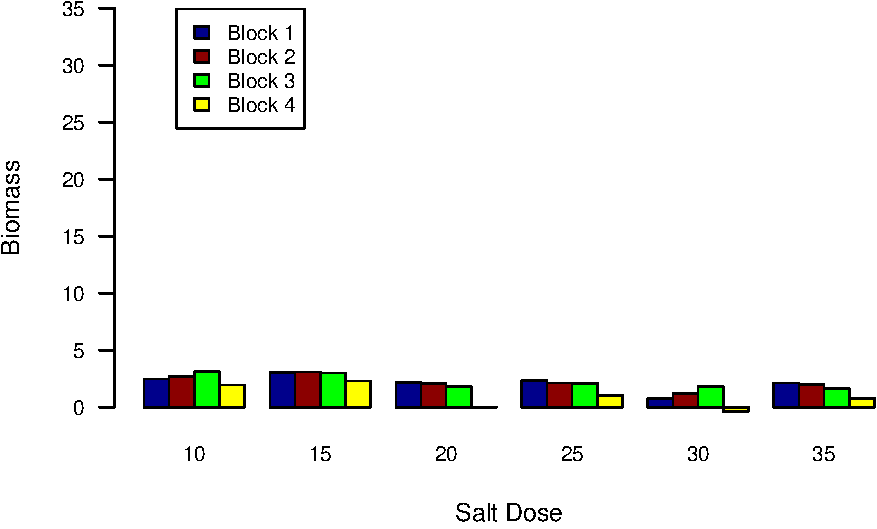
\includegraphics{Neal_Lab_11_files/figure-latex/unnamed-chunk-1-1.pdf}
To determine the correct model, seven different generalized linear
models were created. These models included the saturated model including
all factors, each possible combination of factors, and a model including
only each individual factor. Each reduced model was then compared to the
saturated model with the Likelihood Ratio Test (LRT) in an ANOVA. The
Null Hypothesis of each test is that the reduced model is adequate. The
Alternative Hypothesesis is that the reduced model is not adequate.

\begin{Shaded}
\begin{Highlighting}[]
\NormalTok{dam1 <-}\StringTok{ }\KeywordTok{glm}\NormalTok{(y }\OperatorTok{~}\StringTok{ }\KeywordTok{factor}\NormalTok{(x1) }\OperatorTok{+}\StringTok{ }\NormalTok{x2 }\OperatorTok{+}\StringTok{ }\NormalTok{x3, }\DataTypeTok{family =}\NormalTok{ poisson, }\DataTypeTok{data =}\NormalTok{ dat)}
\NormalTok{dam2 <-}\StringTok{ }\KeywordTok{glm}\NormalTok{(y }\OperatorTok{~}\StringTok{ }\KeywordTok{factor}\NormalTok{(x1) }\OperatorTok{+}\StringTok{ }\NormalTok{x2, }\DataTypeTok{family =}\NormalTok{ poisson, }\DataTypeTok{data =}\NormalTok{ dat)}
\NormalTok{dam3 <-}\StringTok{ }\KeywordTok{glm}\NormalTok{(y }\OperatorTok{~}\StringTok{ }\KeywordTok{factor}\NormalTok{(x1) }\OperatorTok{+}\StringTok{ }\NormalTok{x3, }\DataTypeTok{family =}\NormalTok{ poisson, }\DataTypeTok{data =}\NormalTok{ dat)}
\NormalTok{dam4 <-}\StringTok{ }\KeywordTok{glm}\NormalTok{(y }\OperatorTok{~}\StringTok{ }\NormalTok{x2 }\OperatorTok{+}\StringTok{ }\NormalTok{x3, }\DataTypeTok{family =}\NormalTok{ poisson, }\DataTypeTok{data =}\NormalTok{ dat)}
\NormalTok{dam5 <-}\StringTok{ }\KeywordTok{glm}\NormalTok{(y }\OperatorTok{~}\StringTok{ }\KeywordTok{factor}\NormalTok{(x1), }\DataTypeTok{family =}\NormalTok{ poisson, }\DataTypeTok{data =}\NormalTok{ dat)}
\NormalTok{dam6 <-}\StringTok{ }\KeywordTok{glm}\NormalTok{(y }\OperatorTok{~}\StringTok{ }\NormalTok{x2, }\DataTypeTok{family =}\NormalTok{ poisson, }\DataTypeTok{data =}\NormalTok{ dat)}
\NormalTok{dam7 <-}\StringTok{ }\KeywordTok{glm}\NormalTok{(y }\OperatorTok{~}\StringTok{ }\NormalTok{x3, }\DataTypeTok{family =}\NormalTok{ poisson, }\DataTypeTok{data =}\NormalTok{ dat)}
\KeywordTok{anova}\NormalTok{(dam1, dam2, }\DataTypeTok{test =} \StringTok{"LRT"}\NormalTok{)}
\end{Highlighting}
\end{Shaded}

\begin{verbatim}
## Analysis of Deviance Table
## 
## Model 1: y ~ factor(x1) + x2 + x3
## Model 2: y ~ factor(x1) + x2
##   Resid. Df Resid. Dev Df Deviance Pr(>Chi)
## 1        26     25.953                     
## 2        27     28.634 -1  -2.6812   0.1015
\end{verbatim}

\begin{Shaded}
\begin{Highlighting}[]
\KeywordTok{anova}\NormalTok{(dam1, dam3, }\DataTypeTok{test =} \StringTok{"LRT"}\NormalTok{)}
\end{Highlighting}
\end{Shaded}

\begin{verbatim}
## Analysis of Deviance Table
## 
## Model 1: y ~ factor(x1) + x2 + x3
## Model 2: y ~ factor(x1) + x3
##   Resid. Df Resid. Dev Df Deviance Pr(>Chi)  
## 1        26     25.953                       
## 2        27     32.192 -1  -6.2386   0.0125 *
## ---
## Signif. codes:  0 '***' 0.001 '**' 0.01 '*' 0.05 '.' 0.1 ' ' 1
\end{verbatim}

\begin{Shaded}
\begin{Highlighting}[]
\KeywordTok{anova}\NormalTok{(dam1, dam4, }\DataTypeTok{test =} \StringTok{"LRT"}\NormalTok{)}
\end{Highlighting}
\end{Shaded}

\begin{verbatim}
## Analysis of Deviance Table
## 
## Model 1: y ~ factor(x1) + x2 + x3
## Model 2: y ~ x2 + x3
##   Resid. Df Resid. Dev Df Deviance Pr(>Chi)
## 1        26     25.953                     
## 2        27     27.220 -1  -1.2667   0.2604
\end{verbatim}

\begin{Shaded}
\begin{Highlighting}[]
\KeywordTok{anova}\NormalTok{(dam1, dam5, }\DataTypeTok{test =} \StringTok{"LRT"}\NormalTok{)}
\end{Highlighting}
\end{Shaded}

\begin{verbatim}
## Analysis of Deviance Table
## 
## Model 1: y ~ factor(x1) + x2 + x3
## Model 2: y ~ factor(x1)
##   Resid. Df Resid. Dev Df Deviance Pr(>Chi)   
## 1        26     25.953                        
## 2        28     38.283 -2   -12.33 0.002101 **
## ---
## Signif. codes:  0 '***' 0.001 '**' 0.01 '*' 0.05 '.' 0.1 ' ' 1
\end{verbatim}

\begin{Shaded}
\begin{Highlighting}[]
\KeywordTok{anova}\NormalTok{(dam1, dam6, }\DataTypeTok{test =} \StringTok{"LRT"}\NormalTok{)}
\end{Highlighting}
\end{Shaded}

\begin{verbatim}
## Analysis of Deviance Table
## 
## Model 1: y ~ factor(x1) + x2 + x3
## Model 2: y ~ x2
##   Resid. Df Resid. Dev Df Deviance Pr(>Chi)
## 1        26     25.953                     
## 2        28     29.206 -2  -3.2527   0.1966
\end{verbatim}

\begin{Shaded}
\begin{Highlighting}[]
\KeywordTok{anova}\NormalTok{(dam1, dam7, }\DataTypeTok{test =} \StringTok{"LRT"}\NormalTok{)}
\end{Highlighting}
\end{Shaded}

\begin{verbatim}
## Analysis of Deviance Table
## 
## Model 1: y ~ factor(x1) + x2 + x3
## Model 2: y ~ x3
##   Resid. Df Resid. Dev Df Deviance  Pr(>Chi)    
## 1        26     25.953                          
## 2        28     50.537 -2  -24.584 4.588e-06 ***
## ---
## Signif. codes:  0 '***' 0.001 '**' 0.01 '*' 0.05 '.' 0.1 ' ' 1
\end{verbatim}

\begin{Shaded}
\begin{Highlighting}[]
\KeywordTok{AIC}\NormalTok{(dam1, dam2, dam4, dam6)}
\end{Highlighting}
\end{Shaded}

\begin{verbatim}
##      df      AIC
## dam1  4 87.64922
## dam2  3 88.33037
## dam4  3 86.91589
## dam6  2 86.90196
\end{verbatim}

\begin{Shaded}
\begin{Highlighting}[]
\KeywordTok{summary}\NormalTok{(dam6)}
\end{Highlighting}
\end{Shaded}

\begin{verbatim}
## 
## Call:
## glm(formula = y ~ x2, family = poisson, data = dat)
## 
## Deviance Residuals: 
##     Min       1Q   Median       3Q      Max  
## -1.9188  -1.0473  -0.1518   0.1650   2.6331  
## 
## Coefficients:
##             Estimate Std. Error z value Pr(>|z|)    
## (Intercept) -1.70097    0.50685  -3.356 0.000791 ***
## x2           0.23112    0.04677   4.942 7.72e-07 ***
## ---
## Signif. codes:  0 '***' 0.001 '**' 0.01 '*' 0.05 '.' 0.1 ' ' 1
## 
## (Dispersion parameter for poisson family taken to be 1)
## 
##     Null deviance: 53.883  on 29  degrees of freedom
## Residual deviance: 29.206  on 28  degrees of freedom
## AIC: 86.902
## 
## Number of Fisher Scoring iterations: 5
\end{verbatim}

\begin{Shaded}
\begin{Highlighting}[]
\NormalTok{coef1 <-}\StringTok{ }\KeywordTok{exp}\NormalTok{(}\KeywordTok{coefficients}\NormalTok{(dam6))}
\end{Highlighting}
\end{Shaded}

\paragraph{Results}\label{results}

Based on the results of these comparisons, it is immediately apparent
that the models containing only X1 \& X3 as well as the model with both
X1 \& X3 are not adequate based on .05\textgreater{}p values for each.
This is not surprising given that these factors did not appear to have a
strong correlation upon initial examination of the data. It appears that
all models containing x2 have roughly the same change in residual
deviance, suggesting that these models are essentially the same. To
check this, the AIC criterion for these models was compared and the
value for all was within 2. Therefore, the minimum adequate model
considers only the effects of bomb load on damage: Y = β0 + β1X2 With
the coefficients obtained, the model would be: log(Y) = -1.7 +
.23\emph{X2\\
However, because these values are on a log damage scale, interpretation
is difficult. The model is easier to understand once coefficients are
exponentiated: Y = .183 + 1.26}X2 So, for every 1 ton increase in bomb
load, damage locations will increase by 26\%.

To check for Overdispersion, the diagnostics plots were generated and
examined. Aside from a couple of points that may have exerted too much
leverage in the analysis, the data appear to be fine. Though there are
three points that lie outside of a 1 to -1 standard deviation range,
this is acceptable as roughly 5\% should be expected to lie outside the
range. As a final check, overdispersion was checked and found to be
1.09, indicating normal dispersion. Thus, rejection of the null
hypothesis in favor of a GLM model which related bomb load to damage is
appropriate. This relationshihp is shown in figure 1 below.

\includegraphics{Neal_Lab_11_files/figure-latex/unnamed-chunk-3-1.pdf}
\includegraphics{Neal_Lab_11_files/figure-latex/unnamed-chunk-3-2.pdf}
\#\#Problem 2

\paragraph{Introduction}\label{introduction-1}

The purpose of this analysis is to evaluate the factors that increase
the number of moons associated with terrestrial planets, gas giants, and
dwarf planets in our solar system. Planet size, mass, and distance from
the planet are the regressors. Number of moods is the response variable.
The null hypothesis of this study is that there is no significant
relationship of number of moods to any of the above factors. The
alternative hypothesis is that there is a significant generalized linear
model relationship of number of moons to at least one of the variables
and/or their interactions.

\paragraph{Methods}\label{methods-1}

To visualize the distributions and relationships, the data were plotted
wth ggpairs. Based on this output, number of moons appears to have a
strong positive correlated to planet diameter and mass, with a weak
negative correlation to distance. Planet Diameter and Mass also appear
to have a strong correlation, so the factor with lower significance to
the model will be removed. All data show a strong skew towards lower
values. Based on these distribution, it appears that analysis with GLM
assuming a Poisson distribution is appropriate.

\begin{verbatim}
## Loading required package: Sleuth3
\end{verbatim}

\begin{verbatim}
## `stat_bin()` using `bins = 30`. Pick better value with `binwidth`.
## `stat_bin()` using `bins = 30`. Pick better value with `binwidth`.
## `stat_bin()` using `bins = 30`. Pick better value with `binwidth`.
## `stat_bin()` using `bins = 30`. Pick better value with `binwidth`.
\end{verbatim}

\includegraphics{Neal_Lab_11_files/figure-latex/unnamed-chunk-4-1.pdf}
To determine the correct model, a saturated model was first created
including all factors and their interactions. Diamater and Mass were
then independantly removed to determine which factor is a better fit for
the model. Based on change to AIC and residual variance, Diameter was
chosen to be retained. Again, this is not surprising as this factor
showed a stronger correlation to number of moons in the initial
examination of the data. Finally, because the effects of Distance did
not appear to be significant but the interaction between Distance and
Diameter did, additional models were run in which each parameter was
removed to examine the effects.

\paragraph{Results}\label{results-1}

Based on the AIC for the models, removal of the distance factor does not
change the model, but removal of the interaction does, therefore all
factors will remain in the model. However, when the model was checked
for overdispersion, this was found to be an issue. Therefore, the model
was rerun as a quasi-Poisson model, with the following minimum adequate
model resulting:

Log(Moons) = β0 + β1(Distance) + β2(Diameter) + β2(Distance)(Diameter)

With the coefficients obtained, the model would be: Log(Moons) = .247 +
.002(Distance) + .275(Diameter) + .0143(Distance)(Diameter)

However, because these values are on a log scale, interpretation is
difficult. The model is easier to understand once coefficients are
exponentiated:\\
Log(Moons) = 1.28 + 1.002(Distance) + 1.32(Diameter) +
1.01(Distance)(Diameter)

So, for every 1 unit increase in distance, number of moons will increase
by .2\%. For every 1 unit increase in diameter, number of moons will
increase by 32\%, and for every 1 unit increase in both distance and
diameter, number of moons will increase by 1\%. It is likely that
rescalin the distance data would make this easier to interpret, but
since I don't know the scale of the original it will remain as is.

Diagnostics revealed that data points 8 \& 9 are potentially
problematic. Both points appear to have too much leverage and fall well
outside of an acceptable range for residuals. Were these my actual data,
I would re-examine these data points and consider removal. As a final
step, Moons were plotted as a function of distance and diameter, keeping
the other parameter at a mean value. Because the graph scales made
interpretation difficult, data were plotted as log values.

\begin{verbatim}
## Loading required package: zoo
\end{verbatim}

\begin{verbatim}
## 
## Attaching package: 'zoo'
\end{verbatim}

\begin{verbatim}
## The following objects are masked from 'package:base':
## 
##     as.Date, as.Date.numeric
\end{verbatim}

\begin{verbatim}
## 
## Call:
## glm(formula = Moons ~ Distance + Diameter + Mass + Distance:Diameter + 
##     Diameter:Mass + Distance:Mass, family = poisson, data = dat1)
## 
## Deviance Residuals: 
##      Min        1Q    Median        3Q       Max  
## -1.53913  -1.02283  -0.04556   0.02589   1.97661  
## 
## Coefficients:
##                    Estimate Std. Error z value Pr(>|z|)  
## (Intercept)       -0.759804   1.154290  -0.658   0.5104  
## Distance           0.013042   0.012227   1.067   0.2861  
## Diameter           0.833128   2.664418   0.313   0.7545  
## Mass              -0.006535   1.567339  -0.004   0.9967  
## Distance:Diameter  0.042239   0.057622   0.733   0.4635  
## Diameter:Mass      0.003420   0.128664   0.027   0.9788  
## Distance:Mass     -0.010320   0.005164  -1.999   0.0456 *
## ---
## Signif. codes:  0 '***' 0.001 '**' 0.01 '*' 0.05 '.' 0.1 ' ' 1
## 
## (Dispersion parameter for poisson family taken to be 1)
## 
##     Null deviance: 388.253  on 12  degrees of freedom
## Residual deviance:  13.446  on  6  degrees of freedom
## AIC: 61.462
## 
## Number of Fisher Scoring iterations: 6
\end{verbatim}

\begin{verbatim}
## 
## Call:
## glm(formula = Moons ~ Distance + Mass + Distance:Mass, family = poisson, 
##     data = dat1)
## 
## Deviance Residuals: 
##     Min       1Q   Median       3Q      Max  
## -2.5994  -2.1957  -0.4623   0.1328   5.4126  
## 
## Coefficients:
##                 Estimate Std. Error z value Pr(>|z|)    
## (Intercept)    0.8989277  0.2731831   3.291    0.001 ***
## Distance      -0.0069511  0.0080330  -0.865    0.387    
## Mass          -0.0180306  0.0021266  -8.479   <2e-16 ***
## Distance:Mass  0.0054714  0.0004869  11.237   <2e-16 ***
## ---
## Signif. codes:  0 '***' 0.001 '**' 0.01 '*' 0.05 '.' 0.1 ' ' 1
## 
## (Dispersion parameter for poisson family taken to be 1)
## 
##     Null deviance: 388.253  on 12  degrees of freedom
## Residual deviance:  57.501  on  9  degrees of freedom
## AIC: 99.516
## 
## Number of Fisher Scoring iterations: 6
\end{verbatim}

\begin{verbatim}
## 
## Call:
## glm(formula = Moons ~ Distance + Diameter + Distance:Diameter, 
##     family = quasipoisson, data = dat1)
## 
## Deviance Residuals: 
##     Min       1Q   Median       3Q      Max  
## -1.8941  -1.6885  -0.5906   0.3071   3.6900  
## 
## Coefficients:
##                   Estimate Std. Error t value Pr(>|t|)   
## (Intercept)       0.246706   0.686573   0.359  0.72763   
## Distance          0.001999   0.019685   0.102  0.92133   
## Diameter          0.274679   0.062249   4.413  0.00169 **
## Distance:Diameter 0.014347   0.005492   2.613  0.02815 * 
## ---
## Signif. codes:  0 '***' 0.001 '**' 0.01 '*' 0.05 '.' 0.1 ' ' 1
## 
## (Dispersion parameter for quasipoisson family taken to be 3.567853)
## 
##     Null deviance: 388.253  on 12  degrees of freedom
## Residual deviance:  32.813  on  9  degrees of freedom
## AIC: NA
## 
## Number of Fisher Scoring iterations: 6
\end{verbatim}

\begin{verbatim}
##       df AIC
## moon3  4  NA
## moon4  3  NA
## moon5  3  NA
\end{verbatim}

\includegraphics{Neal_Lab_11_files/figure-latex/unnamed-chunk-5-1.pdf}

\includegraphics{Neal_Lab_11_files/figure-latex/unnamed-chunk-6-1.pdf}

\begin{Shaded}
\begin{Highlighting}[]
\NormalTok{dat <-}\StringTok{ }\KeywordTok{read.csv}\NormalTok{(}\StringTok{"~/710 Lab 11/AircraftDat.csv"}\NormalTok{)}
\KeywordTok{ggpairs}\NormalTok{(dat)}
\NormalTok{dam1 <-}\StringTok{ }\KeywordTok{glm}\NormalTok{(y }\OperatorTok{~}\StringTok{ }\KeywordTok{factor}\NormalTok{(x1) }\OperatorTok{+}\StringTok{ }\NormalTok{x2 }\OperatorTok{+}\StringTok{ }\NormalTok{x3, }\DataTypeTok{family =}\NormalTok{ poisson, }\DataTypeTok{data =}\NormalTok{ dat)}
\NormalTok{dam2 <-}\StringTok{ }\KeywordTok{glm}\NormalTok{(y }\OperatorTok{~}\StringTok{ }\KeywordTok{factor}\NormalTok{(x1) }\OperatorTok{+}\StringTok{ }\NormalTok{x2, }\DataTypeTok{family =}\NormalTok{ poisson, }\DataTypeTok{data =}\NormalTok{ dat)}
\NormalTok{dam3 <-}\StringTok{ }\KeywordTok{glm}\NormalTok{(y }\OperatorTok{~}\StringTok{ }\KeywordTok{factor}\NormalTok{(x1) }\OperatorTok{+}\StringTok{ }\NormalTok{x3, }\DataTypeTok{family =}\NormalTok{ poisson, }\DataTypeTok{data =}\NormalTok{ dat)}
\NormalTok{dam4 <-}\StringTok{ }\KeywordTok{glm}\NormalTok{(y }\OperatorTok{~}\StringTok{ }\NormalTok{x2 }\OperatorTok{+}\StringTok{ }\NormalTok{x3, }\DataTypeTok{family =}\NormalTok{ poisson, }\DataTypeTok{data =}\NormalTok{ dat)}
\NormalTok{dam5 <-}\StringTok{ }\KeywordTok{glm}\NormalTok{(y }\OperatorTok{~}\StringTok{ }\KeywordTok{factor}\NormalTok{(x1), }\DataTypeTok{family =}\NormalTok{ poisson, }\DataTypeTok{data =}\NormalTok{ dat)}
\NormalTok{dam6 <-}\StringTok{ }\KeywordTok{glm}\NormalTok{(y }\OperatorTok{~}\StringTok{ }\NormalTok{x2, }\DataTypeTok{family =}\NormalTok{ poisson, }\DataTypeTok{data =}\NormalTok{ dat)}
\NormalTok{dam7 <-}\StringTok{ }\KeywordTok{glm}\NormalTok{(y }\OperatorTok{~}\StringTok{ }\NormalTok{x3, }\DataTypeTok{family =}\NormalTok{ poisson, }\DataTypeTok{data =}\NormalTok{ dat)}
\KeywordTok{anova}\NormalTok{(dam1, dam2, }\DataTypeTok{test =} \StringTok{"LRT"}\NormalTok{)}
\KeywordTok{anova}\NormalTok{(dam1, dam3, }\DataTypeTok{test =} \StringTok{"LRT"}\NormalTok{)}
\KeywordTok{anova}\NormalTok{(dam1, dam4, }\DataTypeTok{test =} \StringTok{"LRT"}\NormalTok{)}
\KeywordTok{anova}\NormalTok{(dam1, dam5, }\DataTypeTok{test =} \StringTok{"LRT"}\NormalTok{)}
\KeywordTok{anova}\NormalTok{(dam1, dam6, }\DataTypeTok{test =} \StringTok{"LRT"}\NormalTok{)}
\KeywordTok{anova}\NormalTok{(dam1, dam7, }\DataTypeTok{test =} \StringTok{"LRT"}\NormalTok{)}
\KeywordTok{AIC}\NormalTok{(dam1, dam2, dam4, dam6)}
\KeywordTok{summary}\NormalTok{(dam6)}
\NormalTok{coef1 <-}\StringTok{ }\KeywordTok{exp}\NormalTok{(}\KeywordTok{coefficients}\NormalTok{(dam6))}
\KeywordTok{par}\NormalTok{(}\DataTypeTok{mfrow =} \KeywordTok{c}\NormalTok{(}\DecValTok{2}\NormalTok{,}\DecValTok{2}\NormalTok{))}
\KeywordTok{plot}\NormalTok{(dam6)}
\CommentTok{#wont knit with ovrdsp. Dont know why.}
\CommentTok{#ovrdsp(dat$y, dam6)}
\KeywordTok{require}\NormalTok{(ggplot2)}
\KeywordTok{ggplot}\NormalTok{(dat, }\KeywordTok{aes}\NormalTok{(}\DataTypeTok{x =}\NormalTok{ dat}\OperatorTok{$}\NormalTok{x2, }\DataTypeTok{y =}\NormalTok{ dat}\OperatorTok{$}\NormalTok{y)) }\OperatorTok{+}
\KeywordTok{geom_point}\NormalTok{(}\DataTypeTok{shape =} \DecValTok{5}\NormalTok{) }\OperatorTok{+}
\KeywordTok{geom_smooth}\NormalTok{(}\DataTypeTok{method =}\NormalTok{ glm, }\DataTypeTok{color =} \StringTok{"red"}\NormalTok{) }\OperatorTok{+}\StringTok{ }
\StringTok{  }\KeywordTok{xlab}\NormalTok{(}\StringTok{"Bomb Load, tons"}\NormalTok{) }\OperatorTok{+}
\KeywordTok{ylab}\NormalTok{(}\StringTok{"Number of Damage Locations "}\NormalTok{) }\OperatorTok{+}
\StringTok{  }\KeywordTok{labs}\NormalTok{(}\DataTypeTok{caption =} \StringTok{"Figure one.   Bomb Load vs. Damage, With Damage Predicted By: Y = .183 + 1.26*X2                  "}\NormalTok{) }\OperatorTok{+}\StringTok{          }
\KeywordTok{theme_bw}\NormalTok{()}
\KeywordTok{require}\NormalTok{(Sleuth3) }
\NormalTok{dat1 <-}\StringTok{ }\NormalTok{ex2226}
\KeywordTok{attach}\NormalTok{(dat1)}
\KeywordTok{ggpairs}\NormalTok{(dat1)}
\KeywordTok{library}\NormalTok{(lmtest)}
\NormalTok{moon1 <-}\StringTok{ }\KeywordTok{glm}\NormalTok{(Moons }\OperatorTok{~}\StringTok{ }\NormalTok{Distance }\OperatorTok{+}\StringTok{ }\NormalTok{Diameter }\OperatorTok{+}\StringTok{ }\NormalTok{Mass }\OperatorTok{+}\StringTok{ }\NormalTok{Distance}\OperatorTok{:}\NormalTok{Diameter }\OperatorTok{+}\StringTok{ }\NormalTok{Diameter}\OperatorTok{:}\NormalTok{Mass }\OperatorTok{+}\StringTok{ }\NormalTok{Distance}\OperatorTok{:}\NormalTok{Mass, }\DataTypeTok{family =}\NormalTok{ poisson, }\DataTypeTok{data =}\NormalTok{ dat1)}
\NormalTok{moon2 <-}\StringTok{ }\KeywordTok{update}\NormalTok{(moon1,}\OperatorTok{~}\NormalTok{.}\OperatorTok{-}\NormalTok{Diameter }\OperatorTok{-}\StringTok{ }\NormalTok{Diameter}\OperatorTok{:}\NormalTok{Mass }\OperatorTok{-}\StringTok{ }\NormalTok{Diameter}\OperatorTok{:}\NormalTok{Distance )}
\NormalTok{moon3 <-}\StringTok{ }\KeywordTok{update}\NormalTok{(moon1, }\OperatorTok{~}\NormalTok{.}\OperatorTok{-}\NormalTok{Mass }\OperatorTok{-}\StringTok{ }\NormalTok{Mass}\OperatorTok{:}\NormalTok{Distance }\OperatorTok{-}\StringTok{ }\NormalTok{Mass}\OperatorTok{:}\NormalTok{Diameter, }\DataTypeTok{family =}\NormalTok{ quasipoisson)}
\NormalTok{moon4 <-}\StringTok{ }\KeywordTok{update}\NormalTok{(moon3, }\OperatorTok{~}\NormalTok{.}\OperatorTok{-}\NormalTok{Distance)}
\NormalTok{moon5 <-}\StringTok{ }\KeywordTok{update}\NormalTok{(moon3, }\OperatorTok{~}\NormalTok{.}\OperatorTok{-}\NormalTok{Distance}\OperatorTok{:}\NormalTok{Diameter)}
\KeywordTok{summary}\NormalTok{(moon1)}
\KeywordTok{summary}\NormalTok{(moon2)}
\KeywordTok{summary}\NormalTok{(moon3)}
\KeywordTok{AIC}\NormalTok{(moon3, moon4, moon5)}
\NormalTok{coefs1 <-}\StringTok{ }\NormalTok{(}\KeywordTok{coefficients}\NormalTok{(moon3))}
\KeywordTok{par}\NormalTok{(}\DataTypeTok{mfrow =} \KeywordTok{c}\NormalTok{(}\DecValTok{2}\NormalTok{,}\DecValTok{2}\NormalTok{))}
\KeywordTok{plot}\NormalTok{(moon3)}
\CommentTok{#plot describing relationship between Moon Count and Diameter at Mean distance}
\KeywordTok{par}\NormalTok{(}\DataTypeTok{mfrow=}\KeywordTok{c}\NormalTok{(}\DecValTok{1}\NormalTok{,}\DecValTok{2}\NormalTok{), }\DataTypeTok{mar =} \KeywordTok{c}\NormalTok{(}\DecValTok{5}\NormalTok{,}\DecValTok{5}\NormalTok{,}\DecValTok{5}\NormalTok{,}\DecValTok{5}\NormalTok{))}
\NormalTok{x <-}\StringTok{ }\NormalTok{dat1}\OperatorTok{$}\NormalTok{Distance}
\NormalTok{g <-}\StringTok{ }\KeywordTok{mean}\NormalTok{(dat1}\OperatorTok{$}\NormalTok{Diameter)}
\KeywordTok{plot}\NormalTok{(}\DataTypeTok{x =}\NormalTok{ dat1}\OperatorTok{$}\NormalTok{Distance, }\DataTypeTok{y =}\NormalTok{ dat1}\OperatorTok{$}\NormalTok{Moons, }\DataTypeTok{main =} \StringTok{"Moons vs. Distance }\CharTok{\textbackslash{}n}\StringTok{at Mean Diameter"}\NormalTok{, }\DataTypeTok{xlab =} \StringTok{"Log Distance"}\NormalTok{, }\DataTypeTok{ylab =} \StringTok{"Log Moons"}\NormalTok{ )}
\KeywordTok{curve}\NormalTok{((coefs1[}\DecValTok{1}\NormalTok{] }\OperatorTok{+}\StringTok{ }\NormalTok{coefs1[}\DecValTok{2}\NormalTok{]}\OperatorTok{*}\NormalTok{x }\OperatorTok{+}\StringTok{ }\NormalTok{coefs1[}\DecValTok{3}\NormalTok{]}\OperatorTok{*}\NormalTok{g }\OperatorTok{+}\StringTok{ }\NormalTok{coefs1[}\DecValTok{4}\NormalTok{]}\OperatorTok{*}\NormalTok{g}\OperatorTok{*}\NormalTok{x), }\DataTypeTok{add=}\NormalTok{T, }\DataTypeTok{col=}\StringTok{"red"}\NormalTok{)}
\CommentTok{#plot describing relationship between Moon Count and Diameter at Mean distance}
\NormalTok{x <-}\StringTok{ }\NormalTok{dat1}\OperatorTok{$}\NormalTok{Diameter}
\NormalTok{h <-}\StringTok{ }\KeywordTok{mean}\NormalTok{(dat1}\OperatorTok{$}\NormalTok{Distance)}
\KeywordTok{plot}\NormalTok{(}\DataTypeTok{x =}\NormalTok{ dat1}\OperatorTok{$}\NormalTok{Diameter, }\DataTypeTok{y =}\NormalTok{ dat1}\OperatorTok{$}\NormalTok{Moons, }\DataTypeTok{main =} \StringTok{"Moons vs. Diameter }\CharTok{\textbackslash{}n}\StringTok{at Mean Distance"}\NormalTok{, }\DataTypeTok{xlab =} \StringTok{"Log Diameter"}\NormalTok{, }\DataTypeTok{ylab =} \StringTok{"Log Moons"}\NormalTok{ )}
\KeywordTok{curve}\NormalTok{((coefs1[}\DecValTok{1}\NormalTok{] }\OperatorTok{+}\StringTok{ }\NormalTok{coefs1[}\DecValTok{2}\NormalTok{]}\OperatorTok{*}\NormalTok{h }\OperatorTok{+}\StringTok{ }\NormalTok{coefs1[}\DecValTok{3}\NormalTok{]}\OperatorTok{*}\NormalTok{x}\OperatorTok{+}\StringTok{ }\NormalTok{coefs1[}\DecValTok{4}\NormalTok{]}\OperatorTok{*}\NormalTok{h}\OperatorTok{*}\NormalTok{x), }\DataTypeTok{add=}\NormalTok{T, }\DataTypeTok{col=}\StringTok{"blue"}\NormalTok{)}
\end{Highlighting}
\end{Shaded}


\end{document}
